\documentclass[11pt]{amsart}
\usepackage{amssymb,amsmath,booktabs,tikz,hyperref}
\usepackage[margin=1.1in]{geometry}

\newtheorem{theorem}{Theorem}
\newtheorem{proposition}[theorem]{Proposition}
\newtheorem{lemma}[theorem]{Lemma}
\newtheorem{conjecture}[theorem]{Conjecture}
\theoremstyle{definition}
\newtheorem{definition}[theorem]{Definition}
\newtheorem{remark}[theorem]{Remark}
\newtheorem{observation}[theorem]{Observation}

\newcommand{\ad}{\operatorname{ad}}

\title[Alpha-deficits of two-hub trees]{Alpha-deficits of trees with two large stars:\\ computations, a period rule, and conjectures}
\author{Alexandre de Brantes}
\date{Draft, 23 November 2026}

\begin{document}

\begin{abstract}
We study alpha-labellings of trees made of two stars whose centres (hubs) are joined through a small core
tree. When one star grows and the other is fixed, Lemma~5.1 of Brinkmann, Crevals, Melot, Rylands and Steffen
shows that the alpha-deficit eventually becomes constant; we look at the regime where both stars grow, which
lies outside their Theorem~1.2. For every core with at most 9 vertices (635 families, 894{,}701 trees with at
most 62 vertices) the alpha-deficit is at most~1, and in all but five families it becomes constant once both
stars have at least 8 leaves. We prove, with computer assistance, the exact alpha-deficit of two
infinite families over wide ranges of the star sizes: for a star with $t$ leaves hung through one vertex
between the two stars, the deficit is $0$ if $\min(a,b)\le t$ and $1$ otherwise, whenever $\min(a,b)$ is at most
$28,21,17,14,12,10$ for $t=1,\dots,6$; and for a family that contains two of the five exceptions, the boundary between
deficit $0$ and $1$ lies at $a=2b+1$ for exactly those $b$ selected by a rule with period $t$ and a split by $t$
modulo~$3$, which we prove for 128 pairs $(t,b)$ and which passed pre-registered and held-out tests in all
other cases tested. We give one explicit alpha-labelling construction and state the general rules as
conjectures. All code and data are public.
\end{abstract}

\maketitle

\section{Introduction}

A tree $T$ with $n$ vertices and $q=n-1$ edges is \emph{graceful} if there is an injection
$f\colon V(T)\to\{0,\dots,q\}$ whose edge labels $|f(u)-f(v)|$ are exactly $\{1,\dots,q\}$. It is an
\emph{alpha-labelling} (Rosa~\cite{rosa}) if in addition there is a $\lambda$ such that every edge has one end
labelled at most $\lambda$ and the other end labelled more than $\lambda$; then the vertices labelled at most
$\lambda$ form one colour class. Every caterpillar has an alpha-labelling~\cite{rosa}, while no tree of diameter~4
that is not a caterpillar has one~\cite{hkr}. Between these two facts little is known in general; see Gallian's
survey~\cite{gallian}.

Brinkmann, Crevals, Melot, Rylands and Steffen~\cite{bcmrs} introduced the \emph{alpha-deficit} $\ad(T)$, which
measures how far $T$ is from having an alpha-labelling (definition in Section~\ref{sec:prelim}), computed it for all
trees with up to 26 vertices, and proved that adding pendant vertices at a single vertex eventually stops changing
it (Lemma~\ref{lem:51} below). Their Theorem~1.2 uses this to show that, for fixed $k$, the number of trees with
$n$ vertices, maximum degree $n-k$ and given alpha-deficit is constant for $n\ge k^2+k$: one very large star
dominates.

This paper looks at the next regime: \emph{two} large stars. A \emph{two-hub tree} consists of a small core tree
with two marked vertices (hubs), $a$ leaves attached to one hub and $b$ to the other. With $a$ and $b$ both
growing, the maximum degree is about $n/2$, so Theorem~1.2 of~\cite{bcmrs} does not apply, and Lemma~\ref{lem:51}
alone gives constancy in $a$ only for each fixed $b$, with a threshold that grows with $b$.

The work started from super edge-magic labellings: an exhaustive search for super edge-magic labellings of trees
with up to 25 vertices left, as its hardest cases, leafy lobsters made of two large stars joined through a short
connector with one small pendant tree. Alpha-labellings give super edge-magic labellings of trees (one
reverses the labels of one colour class; see~\cite{fim})% TODO: confirm this is the right reference.
, so we asked which of these trees have
alpha-labellings, and found that many do not.

\subsection*{Results}
\begin{itemize}
\item An explicit alpha-labelling of the lobster consisting of two stars joined by a path of length~3 with an
  edge hung on an inner vertex (Proposition~\ref{prop:formula}).
\item Theorem~\ref{thm:conj1}: the exact alpha-deficit of the family $S_t(a,b)$ (Figure~\ref{fig:families}) for
  $t\le 6$ and $\min(a,b)$ up to an explicit bound, proving Conjecture~\ref{conj:1} there. The case $t=1$, $b=4$
  gives a single explicit infinite sequence of trees of diameter~5 with alpha-deficit exactly~1.
\item A census of all two-hub families with cores of at most 9 vertices (Section~\ref{sec:landscape}): the
  alpha-deficit never exceeds~1, and only five families have a boundary between deficit 0 and 1 that moves with
  the size of the other star.
\item Theorem~\ref{thm:period}: for a family containing two of those five, $F_t(a,b)$, the boundary is at $a=2b+1$ exactly for
  the $b$ selected by an explicit rule with period $t$ and a split by $t \bmod 3$; proved for 128 pairs $(t,b)$
  and stated in general as Conjecture~\ref{conj:period}.
\end{itemize}
All theorems except Proposition~\ref{prop:formula} are computer-assisted: they combine Lemma~\ref{lem:51} with
an exhaustive computation of the alpha-deficit below its threshold. Section~\ref{sec:reliability} says what each
computation rests on.

\section{Preliminaries}\label{sec:prelim}

Let $T$ be a tree with colour classes $V_1,V_2$ and $n$ vertices. A \emph{bipartite labelling} is a bijection
$f\colon V(T)\to\{0,\dots,n-1\}$ with $f(V_1)=\{0,\dots,|V_1|-1\}$ (or the same with the classes swapped).
The alpha-deficit is
\[
\ad(T) = (n-1) - \max_f \bigl|\{\,|f(u)-f(v)| : uv\in E(T)\,\}\bigr|,
\]
the maximum taken over bipartite labellings. Thus $\ad(T)=0$ if and only if $T$ has an alpha-labelling.
(Brinkmann et al.\ use labels $1,\dots,n$; the shift changes nothing.)

\begin{lemma}[{\cite[Lemma~5.1]{bcmrs}}]\label{lem:51}
Let $T$ be a tree with colour classes $V_1,V_2$, let $v\in V_1$, and let $T_p$ be $T$ with $p$ pendant vertices
added at $v$. Then $\ad(T_p)=\ad(T_{p'})$ for all $p,p'\ge p_0:=(|V_1|-1)(|V_2|+1)$.
\end{lemma}

So for a family $T_p$ it suffices to compute $\ad(T_p)$ for $p=0,\dots,p_0$ to know it for every $p$. All our proofs
apply this with $v$ the hub carrying $a$ leaves and $T$ the tree with those leaves removed; the bound $p_0$ then
depends on the rest of the tree, which is why each theorem below covers $b$ only up to the point where the
threshold tree has at most 127 vertices.

\section{Two families and the main computed theorems}

\begin{figure}[ht]
\centering
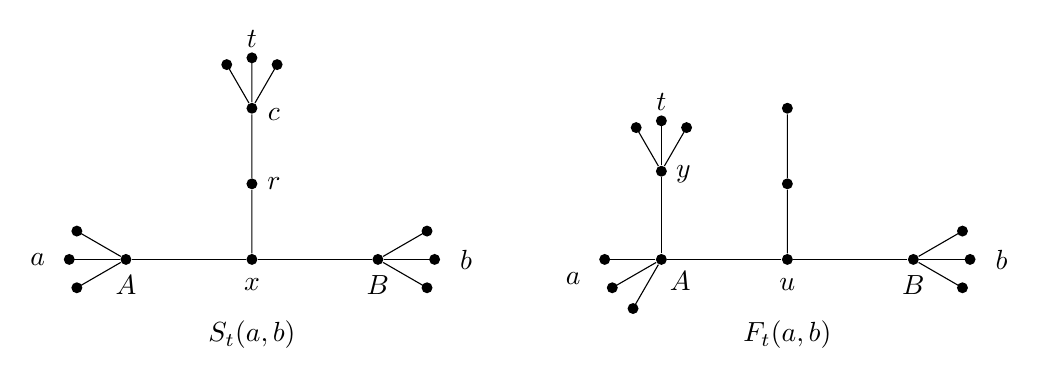
\begin{tikzpicture}[scale=0.8, every node/.style={circle,fill,inner sep=1.4pt}, lab/.style={draw=none,fill=none,rectangle,inner sep=1pt}]
% S_t(a,b)
\node (A) at (0,0) {}; \node (x) at (2,0) {}; \node (B) at (4,0) {};
\node (r) at (2,1.2) {}; \node (c) at (2,2.4) {};
\draw (A)--(x)--(B); \draw (x)--(r)--(c);
\foreach \ang in {150,180,210} \draw (A)--++(\ang:0.9) node {};
\foreach \ang in {-30,0,30} \draw (B)--++(\ang:0.9) node {};
\foreach \ang in {60,90,120} \draw (c)--++(\ang:0.8) node {};
\node[lab] at (-1.4,0) {$a$}; \node[lab] at (5.4,0) {$b$}; \node[lab] at (2,3.5) {$t$};
\node[lab] at (0,-0.4) {$A$}; \node[lab] at (2,-0.4) {$x$}; \node[lab] at (4,-0.4) {$B$};
\node[lab] at (2.35,1.2) {$r$}; \node[lab] at (2.35,2.3) {$c$};
\node[lab] at (2,-1.2) {$S_t(a,b)$};
% F_t(a,b)
\begin{scope}[xshift=8.5cm]
\node (A2) at (0,0) {}; \node (u) at (2,0) {}; \node (B2) at (4,0) {};
\node (w) at (2,1.2) {}; \node (z) at (2,2.4) {};
\node (y) at (0,1.4) {};
\draw (A2)--(u)--(B2); \draw (u)--(w)--(z); \draw (A2)--(y);
\foreach \ang in {180,210,240} \draw (A2)--++(\ang:0.9) node {};
\foreach \ang in {-30,0,30} \draw (B2)--++(\ang:0.9) node {};
\foreach \ang in {60,90,120} \draw (y)--++(\ang:0.8) node {};
\node[lab] at (-1.4,-0.3) {$a$}; \node[lab] at (5.4,0) {$b$}; \node[lab] at (0,2.5) {$t$};
\node[lab] at (0.3,-0.35) {$A$}; \node[lab] at (2,-0.4) {$u$}; \node[lab] at (4,-0.4) {$B$};
\node[lab] at (0.35,1.35) {$y$};
\node[lab] at (2,-1.2) {$F_t(a,b)$};
\end{scope}
\end{tikzpicture}
\caption{The families $S_t(a,b)$ ($n=a+b+t+5$) and $F_t(a,b)$ ($n=a+b+t+6$). Hubs $A$ and $B$ carry $a$ and
$b$ leaves; a third vertex ($c$, resp.\ $y$) carries $t$ leaves.}
\label{fig:families}
\end{figure}

\subsection{An explicit construction}

Let $D(a,b)$ be the tree with path $A\,x_1\,x_2\,B$, $a$ leaves on $A$, $b$ leaves on $B$, and a path $x_1\,r\,s$
hung on $x_1$. It has $n=a+b+6$ vertices and $q=a+b+5$ edges, and for $a,b\ge 1$ it is a lobster that is not a
caterpillar.

\begin{proposition}\label{prop:formula}
For all $a,b\ge 1$, $D(a,b)$ has an alpha-labelling.
\end{proposition}

\begin{proof}
Set $f(A)=0$, $f(r)=1$, $f(x_2)=3$, give $B$'s leaves the labels $\{2\}\cup\{4,\dots,b+2\}$, and set
$f(B)=b+3$, $f(s)=b+4$, $f(x_1)=b+5$; $A$'s leaves get $b+6,\dots,q$. The class of $A$ is
$\{A,r,x_2\}\cup\{\text{leaves of }B\}$ with labels exactly $\{0,\dots,b+2\}$, and every other vertex has a
larger label, so the alpha condition holds with $\lambda=b+2$. The edge labels are: $B$ to its leaves,
$\{1,\dots,b-1\}\cup\{b+1\}$; $x_2B$, $b$; $x_1x_2$, $b+2$; $rs$, $b+3$; $x_1r$, $b+4$; $Ax_1$, $b+5$; $A$ to its
leaves, $b+6,\dots,q$. These are $1,\dots,q$, each once.
\end{proof}

This was found by reading off the lexicographically first labelling from an exhaustive search and checked by
computer for $1\le a\le 60$, $2\le b\le 60$. It is not an instance of Barrientos's gluing lemma~\cite{barrientos}
with star pieces. We have not found it in the literature, but it is a simple lobster and may well be known.

\subsection{The family $S_t(a,b)$}

\begin{conjecture}\label{conj:1}
For all $t,a,b\ge 1$: $\ad(S_t(a,b))=0$ if $\min(a,b)\le t$, and $\ad(S_t(a,b))=1$ otherwise.
\end{conjecture}

\begin{theorem}\label{thm:conj1}
Conjecture~\ref{conj:1} holds for $1\le t\le 6$ whenever $\min(a,b)\le B_t$, where
$(B_1,\dots,B_6)=(28,21,17,14,12,10)$.
\end{theorem}

\begin{proof}[Proof (computer-assisted)]
$S_t(a,b)\cong S_t(b,a)$, so assume $b\le B_t$. Apply Lemma~\ref{lem:51} with $v=A$ and $T=S_t(0,b)$. For every
$t\le 6$ and $b\le B_t$ we computed $\ad(S_t(a,b))$ for every $a=1,\dots,p_0$; the largest of these trees has
127 vertices. All 6{,}026 values agree with the conjecture, and $\ad(S_t(p_0,b))$ is the predicted value for
$a\ge p_0$.
\end{proof}

For $t=1$ and $b=4$ this gives the explicit sequence $S_1(a,4)$ (two stars with $a$ and $4$ leaves through $x$,
and the path $x\,r\,c\,s$): it has an alpha-labelling for $a=1$ and alpha-deficit exactly~1 for every $a\ge 2$.
These trees have maximum degree $n-9$, so by~\cite[Theorem~1.2]{bcmrs} they very likely belong to one of the
``constant series'' that Brinkmann et al.\ enumerated for $k=9$; their lists are not published, so we cannot
confirm this. Their parity obstruction~\cite[Section~4]{bcmrs} does not apply to any tree in the family.

Before Theorem~\ref{thm:conj1}, the conjecture was tested on all $a\ge b\ge 1$ with $n\le 62$ for $t=1,\dots,6$
(4{,}213 trees), without exception. What remains open is the region where both stars exceed $B_t$.

\section{The landscape of two-hub families}\label{sec:landscape}

A \emph{family} is a core tree $C$ with an unordered pair of hubs $h_1,h_2$, considered up to isomorphism; we
require that no leaf of $C$ is adjacent to a hub (except a hub itself), so that hub leaves are exactly the $a$
and $b$ added ones. The trees of the family are $C$ with $a\ge1$ leaves at $h_1$ and $b\ge 1$ at $h_2$.

We computed the alpha-deficit of every tree with at most 62 vertices in every family whose core has at most 9
vertices: 635 families, 894{,}701 trees. Classifying each family by its table of deficits:

\begin{center}
\begin{tabular}{lrl}
\toprule
class & families & description\\
\midrule
ALPHA & 552 & deficit 0 for every $a,b$\\
CONST & 37 & deficit 1 for every $a,b$\\
THRESH & 19 & deficit 0 iff $a\le s_1$ or $b\le s_2$, else 1\\
EVENTUAL & 27 & constant once $a,b\ge m$ for some $m$\\
\bottomrule
\end{tabular}
\end{center}

\begin{observation}
In all 894{,}701 trees the alpha-deficit is at most~1. In 630 of the 635 families the deficit is constant on
all trees with $a,b\ge m$, where $m=1$ for 589 families and $2\le m\le 8$ for the other 41. In the remaining five,
where the deficit switches between 0 and 1 moves with the size of the other star.
\end{observation}

Conjecture~\ref{conj:1} accounts for some of the THRESH families. Two of the five exceptional families have
cores with 8 vertices and three with 9. For the 231 families with cores of at most 8 vertices we checked the
stable regions beyond 62 vertices in two ways: with one hub fixed at $1$ to $6$
leaves and the other at $70$ to $115$ leaves (9{,}958 trees), and with both stars at $30$ to $59$ leaves
(14{,}784 trees, up to 126 vertices). Every tree had the predicted deficit. Boundaries that begin only beyond
about 60 leaves on both stars, families with 9-vertex cores beyond 62 vertices, and cores with more than 9
vertices remain unexamined.

\section{A family with a periodic boundary}\label{sec:period}

Two of the exceptional families are $F_2(a,b)$ and $F_3(a,b)$ of Figure~\ref{fig:families}; the family $F_t$ puts
$t$ leaves on $y$. Computations show that $F_t(a,b)$ has deficit~0 for $a\le 2b$, and for
$a\ge 2b+1$ either deficit~1 throughout (we say $(t,b)$ \emph{has a boundary}) or deficit~0 throughout.
Define
\[
R(t,b) \iff
\begin{cases}
(t\nmid b \text{ and } t\nmid b+2)\ \text{or}\ b=t-2, & t\not\equiv 1 \pmod 3,\\[2pt]
3b\le 2t-5, & t\equiv 1\pmod 3.
\end{cases}
\]
For example, $R(2,b)$ holds iff $b$ is odd, $R(3,b)$ iff $b\equiv 2\pmod 3$ or $b=1$, and $R(1,b)$ never holds.

\begin{conjecture}\label{conj:period}
For all $t,a,b\ge 1$: $\ad(F_t(a,b))=1$ if $R(t,b)$ and $a\ge 2b+1$, and $\ad(F_t(a,b))=0$ otherwise.
\end{conjecture}

\begin{theorem}\label{thm:period}
Conjecture~\ref{conj:period} holds for $1\le t\le 13$ and $1\le b\le B'_t$, for every $a\ge1$, where
$(B'_1,\dots,B'_{13})=(27,20,16,13,11,9,7,6,5,4,4,3,3)$. These are 128 pairs $(t,b)$, of which 61 have a
boundary.
\end{theorem}

\begin{proof}[Proof (computer-assisted)]
Lemma~\ref{lem:51} with $v=A$ and $T=F_t(0,b)$: for each of the 128 pairs we computed every $a=1,\dots,p_0$
(8{,}405 trees, up to 127 vertices) and found the predicted value in each.
\end{proof}

\subsection*{Evidence beyond the proved range, and its provenance}
The rule was first fitted to $t\le 10$ and $b$ up to about 30, at $a=2b,2b+1,2b+4$. A simpler guess,
``$t\nmid b(b+2)$'', fits most of that data but fails at $t=8$ and is separated from $R$ at $t=12$,
$b\equiv 4,6\pmod{12}$. The rule was then frozen in the repository (commit \texttt{eedee92}; the predictions below are commit
\texttt{4306a25}, both dated 14 November 2026, before any of those trees were run) and tested on data it had not
seen:
\begin{itemize}
\item pre-registered predictions for $t=11,12,13$ (30 cases, including the six $t=12$ cases that separate the two
  rules and the $t\equiv 1\pmod 3$ cutoff $b=7$ at $t=13$): 30 of 30 correct;
\item 35 held-out cases from the $t\le 10$ run that finished after the rule was frozen: 35 of 35 correct.
\end{itemize}
The exception $b=t-2$ was read off the data for $t=3,5,6,8,9$; its only fresh tests are $t=11$ ($b=9$) and $t=12$
($b=10$). In total the rule matches all 9{,}259 trees computed for this family (419 pairs $(t,b)$, $t\le 13$, up
to 127 vertices); for the 291 pairs outside Theorem~\ref{thm:period} only $a=2b,2b+1,2b+4$ were computed.

\subsection*{The other three exceptional families}
In each, the hubs are both leaves of the core at a vertex $x$, and a small tree hangs from $x$ through a vertex $p$.
Their rules below are observations, not theorems: they hold for all $a,b$ with $n\le 62$, and the first two
also on samples with up to 126 vertices.
\begin{itemize}
\item $p$ carries two paths of length~2 (core of 8 vertices). For $a\ge b$: alpha iff $b$ is odd, or $b$ is even,
  $a$ is odd and $b<a\le 2b-3$.
\item $p$ carries two leaves and a vertex with two leaves. For $b\ge 5$: if $b$ is odd, deficit 1 iff ($a$ odd and
  $a\ge5$) or $a\ge 2b-2$; if $b$ is even, deficit 1 iff $a$ is odd and $5\le a\le 2\lfloor b/4\rfloor+1$.
\item $x$ also carries a leaf, and $p$ carries a leaf and a vertex with two leaves. For $b\equiv 0,1\pmod 3$
  (from $b=6$) the deficit has period~3 in $a$ up to a cutoff that grows roughly linearly in $b$, and is 1 beyond
  it; for $b\equiv 2\pmod 3$ it is 0 except at $a=3$ and a short run of small $a$ that lengthens with $b$. We
  have not found an exact rule, and this family has not been checked beyond 62 vertices.
\end{itemize}
% TODO: draw these three cores in a figure.

\section{Reliability of the computations}\label{sec:reliability}

Two independent programs were used.
\begin{enumerate}
\item \emph{Our exhaustive search} (\texttt{alpha\_fix.c}) decides whether an alpha-labelling exists, pinning one
  vertex and breaking symmetry between sibling leaves. It was validated against brute force for $n\le 8$,
  against all 557 caterpillars (all alpha) and all 58 diameter-4 non-caterpillars (none alpha~\cite{hkr}) with
  $n\le 12$; every labelling it reports is re-checked from the definition.
\item \emph{Brinkmann's program} \texttt{multi\_alphadeficit}~\cite{bcmrs}, which computes the alpha-deficit and
  is limited to 63 vertices by its 64-bit sets. It agrees with (1) on the number of non-alpha trees for every
  $n=4,\dots,14$ (13{,}402 trees) and tree by tree for $n=13,14$ (4{,}460 trees), and on all 267 two-hub trees
  with $n\le 22$ that we re-decided with (1).
\end{enumerate}
For trees with 64 to 127 vertices we use a 128-bit build of Brinkmann's program, released with his permission
(the change is a compile-time option; the default build is unchanged). It reproduces the original's output on
every tree with $n\le 16$, on 2{,}862 two-hub trees and on 300 random trees with $n\le 62$. On trees above
63 vertices whose answer is known independently it answered all 227 correctly: $S_1(a,4)$ for $n=64,\dots,127$
(deficit 1, by Lemma~\ref{lem:51} and the original program) and 163 random caterpillars (deficit 0); 37 further
caterpillars exceeded a five-minute limit and gave no answer.

\begin{remark}
Of the 128 pairs in Theorem~\ref{thm:period}, 69 do not depend on the 128-bit build: 33 lie within 62 vertices
and were decided by the original program, and in the other 36 every tree above 63 vertices is alpha, with an
explicit alpha-labelling (found by a separate structured search, or produced by the constructive step in the proof
of Lemma~\ref{lem:51}) verified from the definition. The remaining 59
depend on the 128-bit build, 47 of them for non-alpha verdicts (for which we have no certificate) and 12 for
alpha verdicts for which no explicit labelling has been found. Of the 102 pairs in Theorem~\ref{thm:conj1},
38 lie entirely within 63 vertices.
\end{remark}

\section{Open problems}

\begin{enumerate}
\item Prove Conjectures~\ref{conj:1} and~\ref{conj:period} for all star sizes. Both need either a version of
  Lemma~\ref{lem:51} for two vertices with a threshold depending only on the core, or explicit labellings for
  the alpha cases together with an obstruction for the others. In the census the deficit settles after at most
  8 leaves in almost every family, so Lemma~\ref{lem:51}'s bound, which grows with the other star, is far from
  sharp in this setting.
\item Explain the split by $t \bmod 3$ in Conjecture~\ref{conj:period}. Brinkmann et al.\ found alpha-deficit
  $\lfloor m/3\rfloor$ for comets~\cite{bcmrs}; whether that is related is not known.
\item Is the alpha-deficit of every two-hub tree with a core of bounded size at most 1? (It is at most 1 for cores
  with at most 9 vertices and $n\le 62$.)
\item Prove the boundaries of the other moving-boundary families, and decide whether larger cores produce new
  kinds of boundary.
\end{enumerate}

\section*{Data and code}
All scripts, raw outputs and the research log are at
\url{https://github.com/thefullnacho/sem-lobsters}, including the 128-bit build of Brinkmann's program.

\section*{AI assistance}
This work was carried out with extensive help from AI assistants (Claude, by Anthropic) and would not have been
possible without them. They wrote and ran most of the search and analysis code, proposed rules and conjectures and
tested them against the data, found the literature cited here, and drafted this paper. The author directed the
research and decided what to test and what to claim. Every computational claim rests on the programs and checks
described in Section~\ref{sec:reliability}, and all code and raw output are public, so each can be checked
independently; the proof of Proposition~\ref{prop:formula} is short enough to check by hand.

\section*{Acknowledgements}
We thank Gunnar Brinkmann for sending his program \texttt{multi\_alphadeficit} and permitting its release with our
change.

\begin{thebibliography}{9}
% TODO: check every entry against the published version before submission.
\bibitem{barrientos} C.~Barrientos, Alpha-trees over paths and caterpillars, \emph{Utilitas Math.} \textbf{123}
  (2025) 195--204, doi:10.61091/um123-15.
\bibitem{bcmrs} G.~Brinkmann, S.~Crevals, H.~M\'elot, L.~Rylands, E.~Steffen, $\alpha$-labelings and the structure
  of trees with nonzero $\alpha$-deficit, \emph{Discrete Math.\ Theor.\ Comput.\ Sci.} \textbf{14}(1) (2012)
  159--174, doi:10.46298/dmtcs.569.
\bibitem{fim} R.~M.~Figueroa-Centeno, R.~Ichishima, F.~A.~Muntaner-Batle, The place of super edge-magic labelings
  among other classes of labelings, \emph{Discrete Math.} \textbf{231} (2001) 153--168.
\bibitem{gallian} J.~A.~Gallian, A dynamic survey of graph labeling, \emph{Electron.\ J.\ Combin.}, Dynamic Survey
  DS6.
\bibitem{hkr} C.~Huang, A.~Kotzig, A.~Rosa, Further results on tree labellings, \emph{Utilitas Math.} \textbf{21}
  (1982) 31--48.
\bibitem{rosa} A.~Rosa, On certain valuations of the vertices of a graph, in: \emph{Theory of Graphs (Internat.\
  Sympos., Rome, 1966)}, Gordon and Breach, New York, 1967, 349--355.
\end{thebibliography}

\end{document}
